\documentclass[16pt]{beamer}


\usepackage[frenchb]{babel}
\usepackage[T1]{fontenc}
\usepackage[latin1]{inputenc}
\usepackage{ulem}
\usepackage{graphicx}
%\usetheme{theme/beamerthememetropolis}
\usepackage{theme/beamerthememetropolis}

\usepackage{wrapfig}

\title[Code Talkers]{Navajo Code Talkers}
\date{\today}
\author{Am�lie Risi \& Eric Sageloli}

\begin{document}


\begin{frame}
	\maketitle
\end{frame}
% ------------------------------------------------------------------------------------------------

\section{Introduction}
\begin{frame}
    \frametitle{How to secretly send a message?}

    \begin{itemize}
	\item<1-> Steganography %�, hiding the message
	\item<2-> Cryptography %, transforming the message into an apparent nonsense with the possibility to recover the message for selected persons
    \end{itemize}

    \pause
    \pause
      But also..

    \begin{itemize}
	\item Translation of the message into an obscure language
    \end{itemize}
	\begin{figure}
	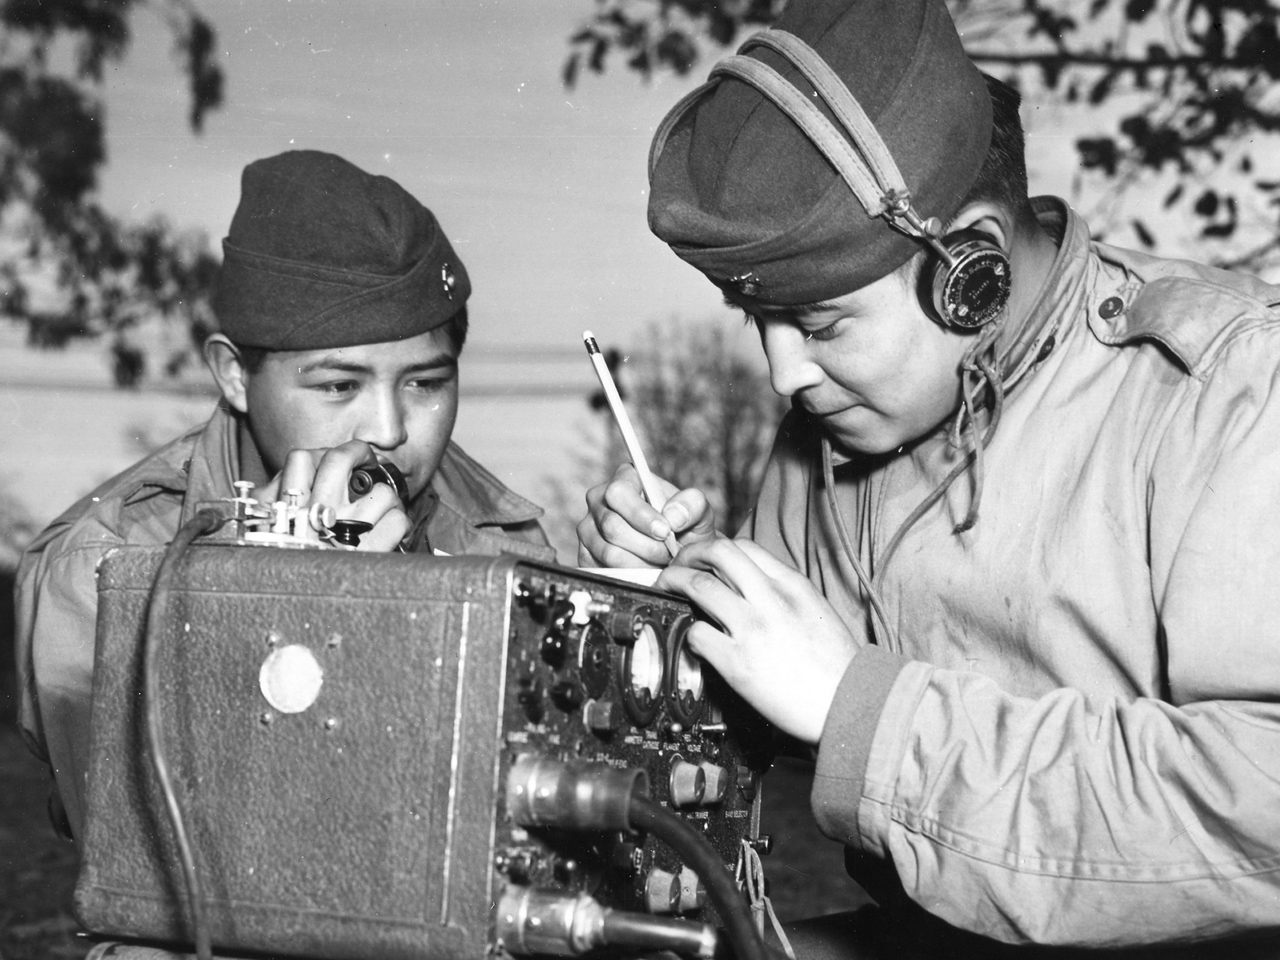
\includegraphics[width=0.5\textwidth]{pictures/title.jpg}
	\end{figure}
\end{frame}
% ------------------------------------------------------------------------------------------------

\begin{frame}
    \frametitle{Code talkers appeared in the first half of 20th century}
    %This method have been used during the first halt of the 20th century by people, called code talkers, who transmit by radio secret messages during wartime.
    %This method was particularly used by America which recruit native
    %American who used their native language.

    Meeting of two conditions:\par
    \begin{itemize}
	\item The existence of the radio and the phone
	\item By that time, most of the cipher machines were too slow and fragile
	to be used for tactical field communications
    \end{itemize}

	\begin{figure}
	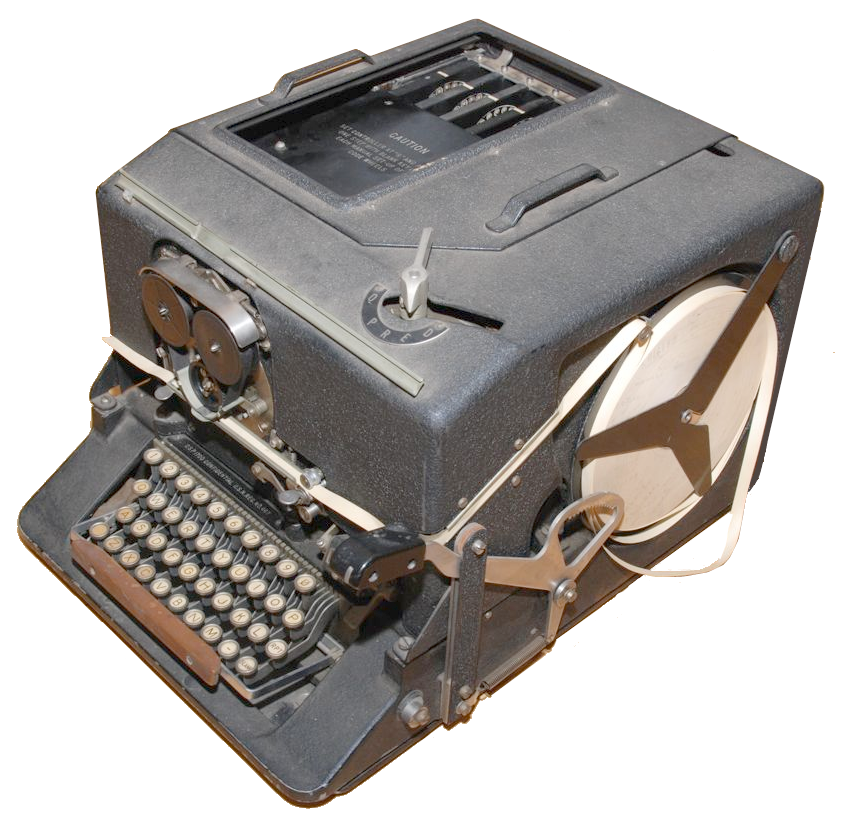
\includegraphics[width=0.3\textwidth]{pictures/SIGABA.png}
	\caption{The SIGABA}
	\end{figure}

\end{frame}
% ------------------------------------------------------------------------------------------------

\begin{frame}
      \frametitle{Plan}

    Plan:
    \begin{itemize}
	\item Relation between the Navajos and the US in the late of the 19th century
	\item How Navajo code talkers have been recruited
	\item Study of the Navajo code
	\item Recognition and current situation of the Navajos
    \end{itemize}
\end{frame}
% ------------------------------------------------------------------------------------------------

\begin{frame}
\section{Navajos and US in the late of the 19th century}


But 
    \begin{itemize}
    \item The long walk
    \item Boarding schools
    \end{itemize}
\end{frame}

\subsection{The Long Walk (1984)}
\begin{frame}
    \frametitle{The long walk}
    In 1864:
    \begin{itemize}
        \item  Deportation of approximately 8000 Navajo people by the
	       government of the United States of America
	\item Forced trek over 480km into the Bosque Redondo camp
    \end{itemize}

    \pause
    They were not informed of:
    \begin{itemize}
	\item Where they were going
	\item Why they were being relocated
	\item How long it would take to get there
    \end{itemize}

    \pause
	\vspace{0.4cm}
    \begin{itemize}
	\item The journey lasted 18 days
	\item Nearly 2000 Navajos died %of exposure to elements and starvations
    \end{itemize}

\end{frame}
% ------------------------------------------------------------------------------------------------

\subsection{Boarding schools }
\begin{frame}
    \frametitle{Boarding schools}

	around 1900:  many American Indian children were in
     church-operated boarding schools

	\begin{figure}
	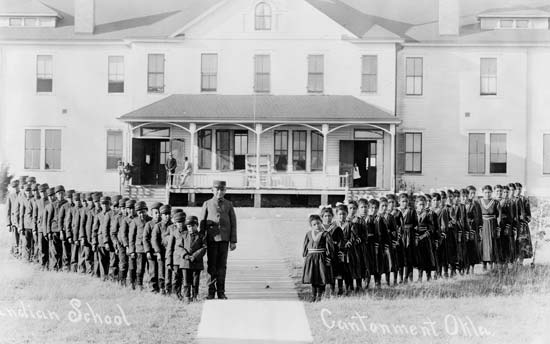
\includegraphics[width=0.5\textwidth]{pictures/boarding_schools.jpg}
	\end{figure}
\end{frame}
% ------------------------------------------------------------------------------------------------

\begin{frame}
    They were forced to
    \begin{itemize}
	\item Speak in English %instead of their native language
	\item Give up their traditional clothing
	\item Drop their native names
	\item Become Christian
    \end{itemize}
	\vspace{1cm}
\end{frame}
% ------------------------------------------------------------------------------------------------


\begin{frame}
\section{Navajos as code talkers: how they have been recruited}
    \begin{itemize}
	\item Preliminary: the code talkers during the WWI
	\item Pacific war and the idea of Philip Johnston
	\item The demonstration
	\item Efficiency of the Navajo code talkers
    \end{itemize}
\end{frame}
% ------------------------------------------------------------------------------------------------

\begin{frame}
    \frametitle{Preliminary: the code talkers during the WWI}
    \begin{itemize}
    \item First use of native American code talkers : Cherokee
    \end{itemize}

    September 1918: During the Second Battle of the Somme, They helped
 	to win the battle
\pause
	\begin{itemize}
		\item After WWI,  Germany sent students and
    anthropologists in America in order to study the various tribal dialects of
    American Indians
	\end{itemize}


\end{frame}
% ------------------------------------------------------------------------------------------------


\begin{frame}
    \frametitle{Pacific war and the idea of Philip Johnston}

    Philip Jonhston
	\begin{figure}
	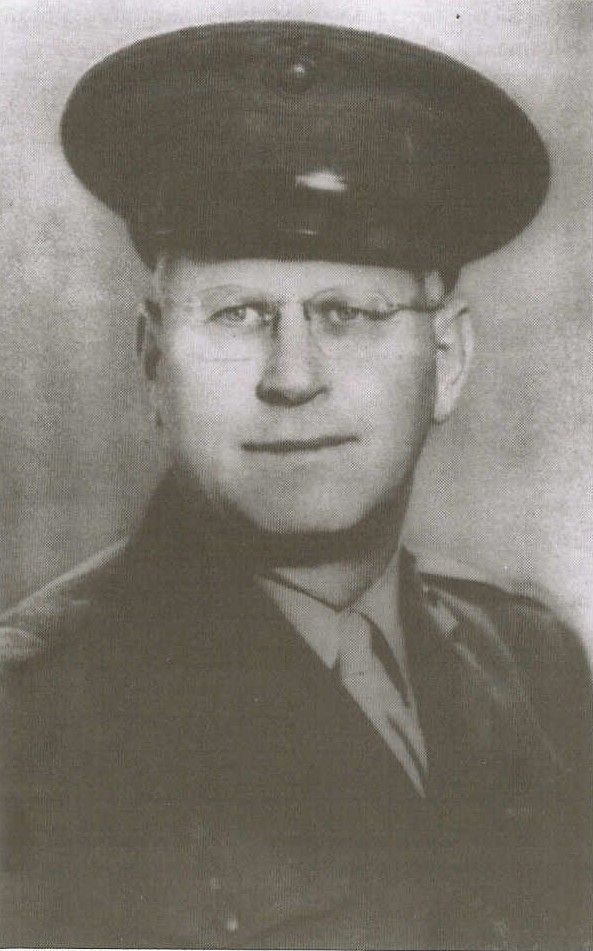
\includegraphics[width=0.13\textwidth]{pictures/Jonhston.jpg}
	\end{figure}

\begin{itemize}
	\item 1942: he proposed to the Marine Corps that Navajos and
    other tribes could be recruited as code talkers

	   \item The major general Clayton
	    Barney Vogel accepted to try the idea
\end{itemize}

\end{frame}
% ------------------------------------------------------------------------------------------------

\begin{frame}
    \frametitle{The demonstration}

    Johnston recruited four bilingual Navajos and % , on February 28,
    they went to Camp Elliott for a demonstration.

    \begin{itemize}
    \item Two of the Navajos translated in Navajo typical military field orders
          and sent it by radio to their companions
    \item The companions translated the message in English
    \end{itemize}
\end{frame}
% ------------------------------------------------------------------------------------------------


\begin{frame}
    Example,

    \begin{quote}
    "Enemy expected to make tank and dive bomber attack at dawn."
    \end{quote}

    becomes...
    \pause
    \begin{quote}
    "Enemy tank dive bomber expected to attack this morning."
    \end{quote}
\pause
    Translation was done in 20 second instead of the 30 minutes needed by machines at that time.
\end{frame}
% ------------------------------------------------------------------------------------------------


\begin{frame}

    \begin{itemize}
    \item May 1942: 29 Navajo code talkers are recruited 
    \item Altogether, between 375 to 420 Navajos participated to the program.
    \end{itemize}

    %![the letter](pictures/letter.jpg)
\end{frame}

\begin{frame}
\section{Navajo and Navajo code}
    \begin{itemize}
	\item Why the Navajo language was a good choice
	\item How it works
	\item Evolution of the code
	\item Some flaws of the code
        \item Efficiency of the Navajo code talkers
    \end{itemize}
\end{frame}
% ------------------------------------------------------------------------------------------------

\begin{frame}
	\frametitle{Why the Navajo language was a good choice?}
    	\begin{itemize}
	  % In addition to what Eric already said, the  OBLIGATOIRE


	% In addition, because Navajo are ...
	\item<1-> The largest population of Native American
	  % officiers had the possibility to recruit enough
          % Navahos code talkers.  OBLIGATOIRE

	  % Then, as Eric mentioned, Navaho language was obscure
          % because only a handful of non Navajo were able
          % to speak it. Moreover, it remained mostly unwritten
	  % and thus was difficult to study
	\item<2-> It remained mostly "unwritten"

	  % The code is also secure because the Navaho grammar
	  %  is complex and different from the German and Japanese one.
 	\item<3-> Complex grammar
		
	\item<4-> Imposture aren't easy to make
          % And above all, it is difficult to pretend to be a Navaho 
	  % if you don't have a good accent. 
    \end{itemize}
\end{frame}
% ------------------------------------------------------------------------------------------------

\begin{frame}
    \frametitle{How it works}

    % We just saw that Navaho was a good choice but it couldn't be used
    % directly because of a lack of military terms. As a consequence, 
    % the code talkers have created a code. OBLIGATOIRE

    % It consists in two parts; the first one is a dictionnary for common
    % military words
    Because of a lack of military terms, a code was needed.
    \pause
    \begin{itemize}
	\item Dictionary for common military words
    \end{itemize}
    % parler de l'usage de poissons pour bateaux/ oiseaux pour avions, qui
    % ressemblent aux appareils (usage de m�taphores?)
\begin{center}
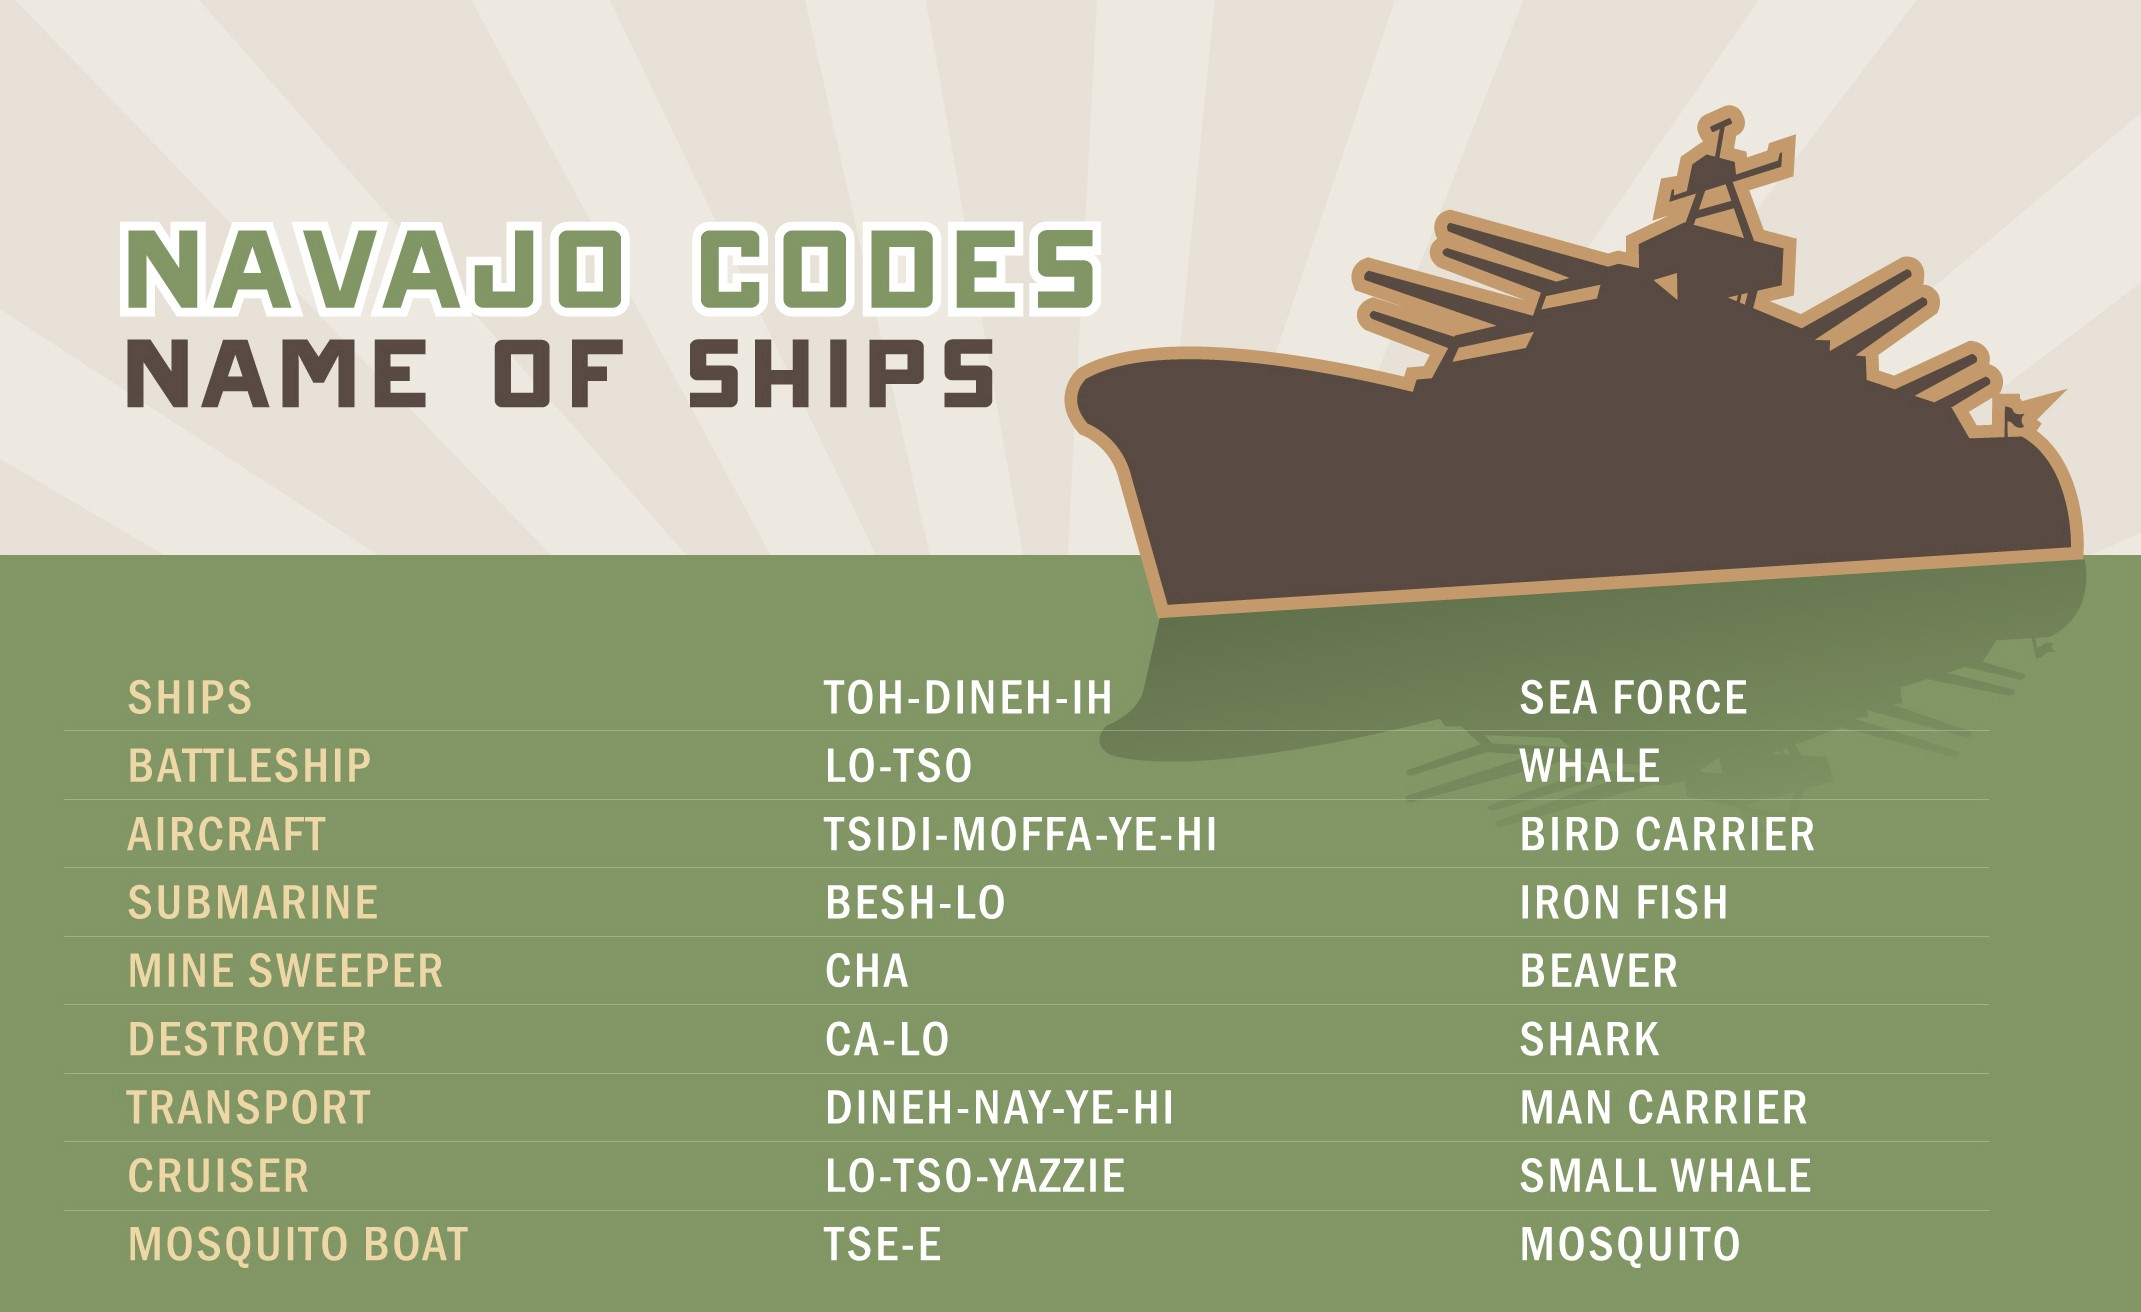
\includegraphics[width=0.7\textwidth]{pictures/ships.jpg} \newline
    \tiny{https://www.cia.gov/news-information/featured-story-archive/2008-featured-story-archive/navajo-code-talkers/}
\end{center}
\end{frame}
% As you can see, they named ships with fish's names

% ------------------------------------------------------------------------------------------------

\begin{frame}
    \frametitle{How it works}
    % The second one is a phonetic alphabet used for words 
    % that are not in the dictionary or in the Navaho langage. 

    % To make it, the logical choice would be to associate each letter
    % with a Navaho word beginning with this letter. However, the Navaho
    % doesn't have the same alphabet so, as you can see, each letter is 
    % associated to an English word which is translated in Navaho        OBLGATOIRE

    \begin{itemize}
    \item A phonetic alphabet table
    \end{itemize}

\begin{center}
    \begin{figure}[H]
\begin{tabular}{c|c|c}
\hline
A & Ant & WOL-LA-CHEE \\
\hline
B & Badger & NA-HASH-CHID \\
\hline
C & Cat & MOASI\\
\hline
D & Devil & CHINDI\\
\hline
E & Ear & AH-JAH \\
\hline
F & Fox &  MA-E \\
\hline
\end{tabular}
	\caption{correspondance for some letters}
\end{figure}
	\tiny
	{https://www.cia.gov/news-information/featured-story-archive/2008-featured-story-archive/navajo-code-talkers/ }
\end{center}
% At the end,, they needed to memorize 17 pages of code.
% It was easy for them because of their oral culture.  % OBLIGATOIRE

\end{frame}
% ------------------------------------------------------------------------------------------------

\begin{frame}
  \frametitle{Evolution of the code}
  % The navaho code talkers have extended the code after its creation,
  % for example:  OBLIGATOIRE

    \begin{itemize}
	\item The original dictionary of 211 terms has been progressively
	expanded to 411
  %  they expanded the phonetic alphabet in order to have multiple words
  %  corresponding to one letter. 
	\item  Multiple words to spell one letter
    \end{itemize}

    \begin{center}
    \begin{figure}
    \begin{tabular}{c|c|c}
	\hline
	A & Ant &  WOL-LA-CHEE  \\
	\hline
	A &  Apple & BE-LA-SANA \\
	\hline
	A & Axe & TSE-NILL \\
	\hline
    \end{tabular}
	\caption{multiple correspondances for one letter}
    \end{figure}
	\tiny
	{https://www.cia.gov/news-information/featured-story-archive/2008-featured-story-archive/navajo-code-talkers/ }
    \end{center}
\end{frame}
% ------------------------------------------------------------------------------------------------


\begin{frame}
  \frametitle{Some flaws of the code}
  % However, the code steal have some flaw. Indeed, Kerchhoff's principles ...
    Modern standards not respected:
    \begin{itemize}
	\item<1-> Non uniqueness of the translations of a message
		% So it can't be a crypto-system OBLIGATOIRE
    \item<2-> Kerckhoffs's principles aren't observed
      % Indeed, the secret lives in the secrecy of the Navaho language and the
      % navaho code
      % So, if a code talker  talks to the enemy, the code is broken.
    \end{itemize}
    On the field:
    \begin{itemize}
	\item<3-> Different evolutions of the code appeared
		% Different evolutions of the code appeared in different places
		% and they didn't have the time to exchange them.
		% OBLIGATOIRE

	\item<4-> Some battalions didn't have code talkers
		% so they were not able  to decrypt and encrypt messages.
		% OBLIGATOIRE
    \end{itemize}



\end{frame}
% ------------------------------------------------------------------------------------------------


\begin{frame}
    \frametitle{Efficiency of the Navajo code talkers}
 
    Battle of Iwo Jima (1945):
	\begin{itemize}
	\item Six Navajo Code Talkers sent more than 800 messages. 
		% All were transmitted without error.
    \end{itemize}
\begin{quote}
" Were it not for the Navajos, the Marines would never have taken Iwo Jima."
	\par
Major Howard Connor, signal officier of the Navajos at Iwo Jima
\end{quote}
	      
	      \pause
	\begin{itemize}
	\item They also served during the Korean War and Vietnam War. 
\pause
% According to the NY times
\item  The only spoken military code
never to have been deciphered.
	\end{itemize}

\end{frame}
% ------------------------------------------------------------------------------------------------


\begin{frame}
\section{Conclusion:}
    \begin{itemize}
	\item Recognition of Navajo code talkers
	\item Current situation
    \end{itemize}
\end{frame}
% ------------------------------------------------------------------------------------------------

\begin{frame}
  % To conclude, we will focus on what happened to the Navajo after the war  
  \frametitle{Recognition of Navajo code talkers}
 Vietnam War : End of the use of Navajo code talkers 
	\begin{itemize}
		\item Declassification of the program (1968)
		%\item A possible cause was that cipher machines had become more efficient
	\end{itemize}
	
Beginning of recognition of code talkers
% It take some time but finally, they received public honors from the
% government.   % OBLIGATOIRE

  \begin{itemize}
  \item 1982: Certificate of Recognition
  \item 2000: they received medals from the US Congree
  \item 2008: signature of the Code talkers recognition
  \end{itemize}
\end{frame}
% ------------------------------------------------------------------------------------------------

\begin{frame}
    \frametitle{Current situation}
  %So, we see that the current situation of Navahos is better than it was 
  %in the past but they are still facing a lot of problems. OBLIGATOIRE

  \begin{itemize}
  \item Poor conditions life
  \begin{itemize}
	  \item Unemployment
		% Unemployement rate higher than the average
	  \item Health problems
    % They live close to ancient uranium mines and it is the cause of severe
  % health problems. 
  \end{itemize}
  \item There is still some lack of respect
    %In 2017, during event intended to honor the Navajo
    %code talkers, Trump used the nickname "Pocahontas" to deride Elizabeth
    %Warren, a political opponent.
  \end{itemize}

\begin{center}
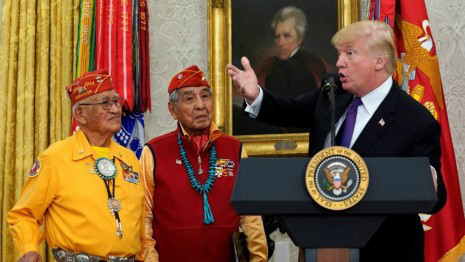
\includegraphics[width=0.7\textwidth]{pictures/trump.jpeg} \newline
\tiny{https://warriorpublications.files.wordpress.com/2017/11/trump\_navajo.jpg?w=604}
\end{center}

\end{frame}
% ------------------------------------------------------------------------------------------------

\begin{frame}
    \frametitle{Sources used}
    \begin{itemize}
    \item  https://www.archives.gov/education/lessons/code-talkers
    \item https://navajocodetalkers.org/
    \item https://www.cia.gov/news-information/featured-story-archive/2008-featured-story-archive/navajo-code-talkers/
    \item https://en.wikipedia.org/wiki/Code\_talker
    \item http://www.historynet.com/world-war-ii-navajo-code-talkers.htm
    \item https://www.nytimes.com/2014/06/06/us/chester-nez-dies-at-93-his-native-tongue-helped-to-win-a-war-of-words.html?\_r=0)
    \end{itemize}
\end{frame}
% ------------------------------------------------------------------------------------------------

\begin{frame}

\begin{center}
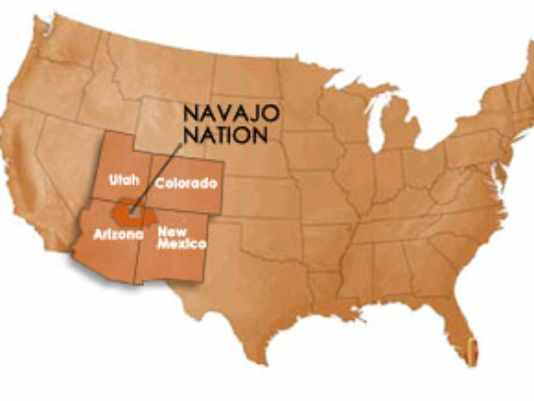
\includegraphics[width=0.7\textwidth]{pictures/navahos.jpeg} \newline
\end{center}

\end{frame}
% ------------------------------------------------------------------------------------------------

\end{document}
